\section{Study region and benchmark design}\label{sec:design}

\subsection{Study region}\label{sec:region}
Northeast Thailand (Isan) comprises 20 provinces on the Khorat Plateau, bounded by the Mekong River to the north and east, the Phetchabun range to the west and the Dangrek range to the south (Fig.~\ref{fig:thailand}a,b). The plateau is drained by the Chi and Mun rivers, which join before flowing into the Mekong. Most rice in the region is grown as a single rainfed wet-season crop on light-textured, often sandy soils, parts of which are affected by salinity, and upland fields are increasingly planted with cassava and sugarcane. The monsoon delivers most rainfall between May and October, with a drier, rain-shadowed south-west and a wetter north-east, so that early-season dry spells, an early end of the rains and floods along the river systems dominate the year-to-year variability of yields.

The benchmark reproduces these features qualitatively (Sections~\ref{sec:design-spatial}--\ref{sec:design-sat}) but contains no observed data from the region. To relate the simulation to real geography, each simulated district is assigned to the province of its nearest provincial capital and district values are averaged by province. Fig.~\ref{fig:thailand}c--f shows the simulated satellite signal at this level for four seasons. In \mapYearA{} and \mapYearC{}, the two shock seasons of the test period, peak-season greenness was below normal in \mapNegA{} and \mapNegC{} of the \mapNprov{} provinces (regional means $\mapAnomA$ and $\mapAnomC$), whereas in \mapYearB{} and \mapYearD{} it was above normal in \mapPosB{} and \mapPosD{} provinces (regional means $\mapAnomB$ and $\mapAnomD$). The spatial patterns differ between seasons---the \mapYearA{} deficit is concentrated in the north-west of the region and the \mapYearC{} deficit in the west and south-west---reflecting the spatially correlated rainfall anomalies of the data-generating process; a model that is to be useful must therefore resolve within-region contrasts, not only the regional mean.

\begin{figure}[tbp]\centering
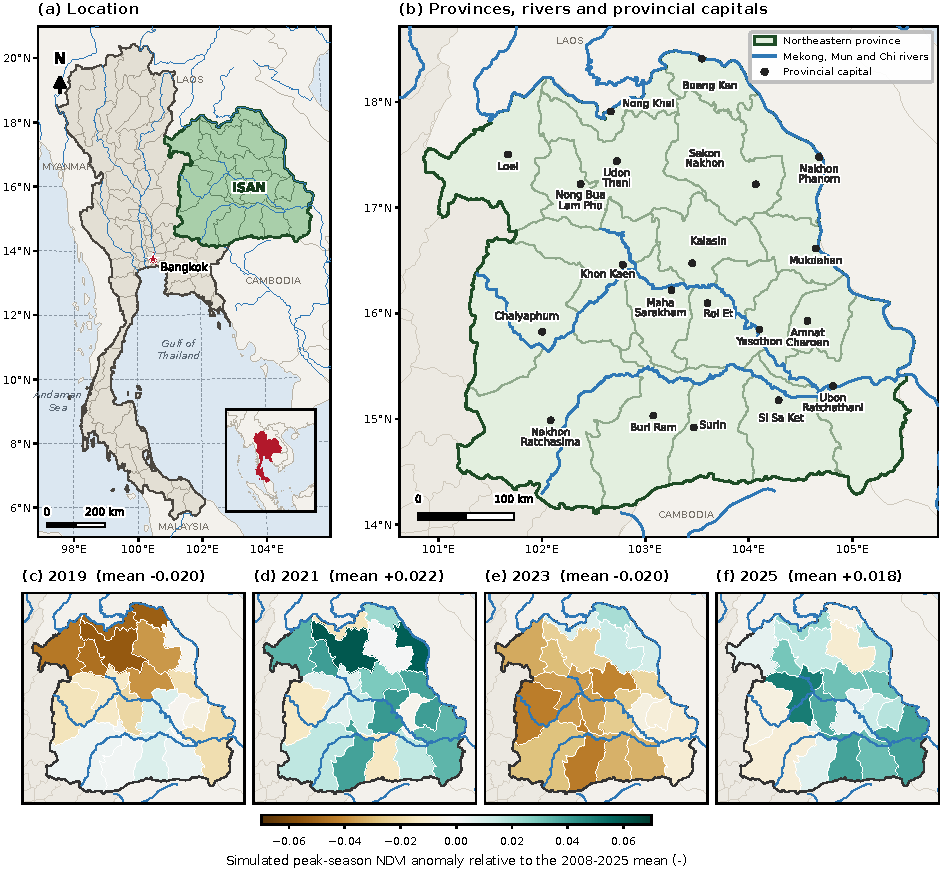
\includegraphics[width=\textwidth]{fig_thailand}
\caption{Study region. (a) Northeast Thailand (Isan; green) within Thailand and Southeast Asia (inset); star: Bangkok. (b) The 20 northeastern provinces with the Mekong, Mun and Chi rivers and the provincial capitals. (c--f) Simulated peak-season NDVI anomaly, relative to each simulated district's 2008--2025 mean and averaged over the simulated districts of each province, in four seasons (panel titles give the regional mean); these are benchmark values, not satellite observations. Boundaries and rivers: Natural Earth \citep{naturalearth}; projection WGS~84 / UTM zone 47N (EPSG:32647).}\label{fig:thailand}
\end{figure}

\subsection{Forecasting problem}
The unit of analysis is a district (\emph{amphoe}) $i$ in season $t$; the target $y_{it}$ is the main-season rice yield in \kgrai{} (1~rai $=0.16$~ha, hence 1~\kgrai{} $=6.25$~kg\,ha$^{-1}$). The season runs from sowing in May to harvest in November and is divided into establishment (May--July), vegetative (August--September) and reproductive (October--November) stages. A forecast for season $t$ issued at the end of month $\tau$ may use any information available by then: yields of earlier seasons, weather and satellite observations up to $\tau$, prices observed before sowing, and static map layers.

\subsection{Design of the simulation study}
We follow the aims--data-generating mechanisms--estimands--methods--performance structure recommended for simulation studies \citep{morris2019using}. The aims are RQ1--RQ4. The data-generating mechanisms are described below, in Table~\ref{tab:dgp} and in Appendix~\ref{app:dgp}. The estimands are out-of-sample forecast errors on the test seasons 2018--2025 and, for RQ3, the true additive yield components. The methods are the learners and protocols of Section~\ref{sec:methods}, and performance is measured by the error, coverage and recovery statistics of Section~\ref{sec:metrics}. The main world uses seed 42; ten further worlds and four scenario worlds quantify Monte-Carlo and structural variability (Section~\ref{sec:robustness}).

\subsection{Spatial layers}\label{sec:design-spatial}
District centroids are placed inside an outline of the region with Mitchell's best-candidate algorithm, which yields an even, administrative-like spacing; Voronoi cells are used only for display (Fig.~\ref{fig:study}). Static layers combine smooth deterministic patterns with spatially correlated Gaussian random fields (kernel-smoothed white noise with length scales of 40--150~km): elevation with the Phetchabun, Dangrek and Phu Phan uplands and lower river valleys; slope; soil sand content, soil organic carbon (SOC) and pH; salinity hot spots in the central lowlands; a four-class land-suitability index (S1, S2, S3, N); irrigated and paddy shares; flood frequency, which decays with distance from the Mekong, Mun and Chi; and distances to provincial towns (markets) and sugar mills. The observed sand, SOC, salinity and irrigation layers equal the true values plus measurement error, mimicking coarse soil maps and outdated irrigation inventories.

\subsection{Weather, water and soil moisture}
A season-level, ENSO-like index $e_t$ (positive: dry and hot) loosely follows the historical phase sequence \citep{ropelewski1987global}. Monthly rainfall is log-normal around a district rainfall normal that increases from the rain-shadowed south-west to the wet north-east, with seasonal, monthly and idiosyncratic spatially correlated anomalies; dry phases depress June--July rainfall most. Temperature follows a lapse rate, a warming trend, $e_t$ and rainfall anomalies, and relative humidity rises with rainfall. Soil moisture follows a texture-dependent bucket model, so that identical rainfall leaves sandy soils drier. Reservoir storage at sowing in each of three basins depends on the previous season's dryness and supplies water to irrigated areas.

\subsection{Prices and economic behaviour}
National farm-gate prices of rice, cassava, sugarcane, maize and urea follow correlated log-AR(1) processes with occasional shocks such as fertiliser price spikes. Local prices subtract transport costs proportional to the distance to a market or, for cane, to a sugar mill. Two behavioural channels act on yields through lag-1 prices known at sowing: a higher rice-to-urea price ratio raises input intensity, and a higher revenue of competing crops relative to rice diverts labour and inputs from rice, more strongly in non-irrigated districts. A harvest-to-price feedback lowers the rice price in seasons with a large regional harvest, so that same-season prices carry information about the season's yields---a realistic source of endogeneity that the leakage audit exploits.

\subsection{Yield equation}
Yield is the clipped sum of additive components,
\begin{equation}\label{eq:yield}
y_{it} = \min\Big\{850,\ \max\big\{120,\ b_i + \tau\,(t-2008) + D_{it} + F_{it} + H_{it} + R_{it} + S_{it} + P_{it} + m_{it} + \pi_{it} + \varepsilon_{it}\big\}\Big\},
\end{equation}
where $b_i$ is a district base level, $D$ drought (establishment and late season), $F$ flood, $H$ heat, $R$ humid-season disease, $S$ salinity aggravated by drought, $P$ price effects, $m$ an AR(1) management effect, $\pi$ local pest outbreaks and $\varepsilon$ unobservable noise (Table~\ref{tab:dgp}). All stress terms are hinge functions, which creates non-linearity, and several are interactions (irrigation~$\times$~reservoir buffering, salinity~$\times$~drought, competition~$\times$~irrigation). Pest outbreaks occur in \pestYears{} and affect districts within roughly 70~km of a random centre; they are visible to the satellite indices but to no weather variable.

\subsection{Satellite observation model}\label{sec:design-sat}
Monthly NDVI follows a bell-shaped seasonal curve whose amplitude saturates in the \emph{visible} part of yield (all components except $\varepsilon$) and whose peak is delayed when early-season soil moisture is low; flooding depresses NDVI in September--October. EVI responds less saturatingly, LSWI tracks soil moisture, transplanting water and floods, and LST rises with maximum temperature and dryness and falls with greenness. Monsoon clouds remove or contaminate monthly composites with month-specific probabilities of up to 50\% in August; contamination lowers the vegetation indices and LST, as in real composites.

\subsection{Ground truth and scenarios}
For every district-season the simulator stores the true components of Eq.~\eqref{eq:yield}. Four scenario variants of the main world test structural robustness: (a) stronger non-linearity (all threshold terms multiplied by 1.8 plus a compound heat--drought penalty), (b) three-fold map-layer measurement error, (c) 1.7-fold cloud contamination, and (d) no pest outbreaks, that is, no satellite-only signal.

\begin{table}[t]\centering\scriptsize
\caption{Additive yield mechanisms of the benchmark DGP (contributions in kg\,rai$^{-1}$), parameter values used in the base world, and the feature groups that observe each mechanism. $q_i$: soil-quality index; $I_i$: irrigated share; $\bar s$: true soil moisture (JJ: Jun--Jul, SO: Sep--Oct); $S_{it}$: irrigation supply (irrigated share $\times$ reservoir storage); $f_i$: flood frequency; $w_{it}$: Aug--Sep rainfall relative to normal; $\sigma_i$: saline share; $\tilde c_{it}$, $\tilde p_{it}$: standardised competing-revenue and rice/urea indices from lag-1 local prices; $\bar a_t$: regional mean yield anomaly. Scenario variants multiply all threshold terms by 1.8 and add a compound heat--drought penalty (non-linear), triple map-layer measurement error, raise cloud frequency 1.7-fold, or remove pests.}\label{tab:dgp}
\begin{tabularx}{\textwidth}{@{}p{2.3cm}Xp{3.9cm}p{2.3cm}@{}}
\toprule
Mechanism & Contribution to $y_{it}$ & Parameters & Observed by \\
\midrule
Base level & $b_i=\beta_0+\beta_q q_i+\beta_I I_i+\sigma_u u_i+\sigma_\eta\eta_i$ & $\beta_0=365$, $\beta_q=30$, $\beta_I=115$, $\sigma_u=18$, $\sigma_\eta=12$ & Geography, map, history \\
Technology trend & $\tau\,(t-2008)$ & $\tau=2.2$ & History \\
Establishment drought & $-\gamma_E\max\{0,\theta_E-(\bar s^{JJ}_{it}+\kappa_E S_{it})\}$ & $\gamma_E=1100$, $\theta_E=0.24$, $\kappa_E=0.12$ & Moisture, water, satellite \\
Late-season drought & $-\gamma_L\max\{0,\theta_L-(\bar s^{SO}_{it}+\kappa_L S_{it})\}$ & $\gamma_L=900$, $\theta_L=0.22$, $\kappa_L=0.1$ & Moisture, water, satellite \\
Flood & $-\min\{c_F,\ \gamma_F (f_i/0.3)\max(0,w_{it}-\theta_F)\}$ & $\gamma_F=160$, $\theta_F=1.3$, $c_F=150$ & Water, map, satellite \\
Heat at flowering & $-\gamma_H\sum_{m\in\{9,10\}}\max(0,T^{\max}_{itm}-\theta_H)$ & $\gamma_H=6$, $\theta_H=34$\,$^\circ$C & Climate \\
Humid-season disease & $-\gamma_D\max(0,\overline{RH}^{AS}_{it}-\theta_D)$ & $\gamma_D=4$, $\theta_D=84$\,\% & Moisture \\
Salinity $\times$ drought & $-\gamma_S\,\sigma_i\max(0,\theta_S-\bar s^{JJ}_{it})$ & $\gamma_S=250$, $\theta_S=0.26$ & Geography, moisture \\
Prices \& competition & $-\gamma_C\,\tilde c_{it}(1-I_i)+\gamma_P\,\tilde p_{it}(0.6+I_i)$ & $\gamma_C=12$, $\gamma_P=10$ & Prices, map \\
Harvest-price feedback & $\ln P^{\mathrm{rice}}_t \leftarrow \ln P^{\mathrm{rice}}_t-\kappa\,\bar a_t/100$ & $\kappa=0.25$ & (price endogeneity) \\
Management & $m_{it}=\rho\,m_{i,t-1}+\sigma_m\xi_{it}$ & $\rho=0.6$, $\sigma_m=14$ & History, satellite \\
Pest outbreaks & $-A\exp\{-d_{ic}^2/(2r^2)\}$ in 3 seasons & $A=75$, $r=70$\,km & Satellite only \\
Noise & $\varepsilon_{it}\sim\mathcal N(0,\sigma_\varepsilon^2)$ & $\sigma_\varepsilon=16$ & None (irreducible) \\
\bottomrule
\end{tabularx}
\end{table}

\begin{figure}[t]\centering
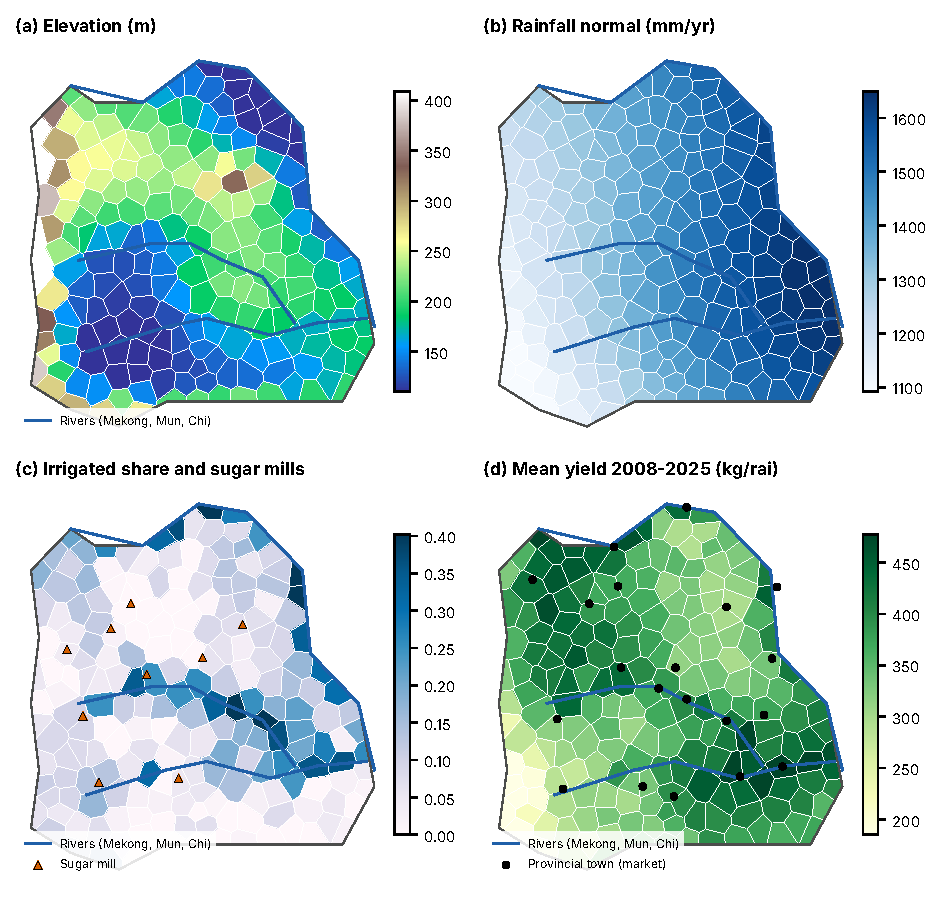
\includegraphics[width=\textwidth]{fig1_study_area}
\caption{The synthetic study region (main world, \nDistricts{} districts; Voronoi cells for display only). (a) Elevation; (b) rainfall normal; (c) observed irrigated share and sugar mills; (d) mean simulated yield 2008--2025 and the provincial towns used as markets. Blue lines: simplified Mekong, Mun and Chi rivers.}\label{fig:study}
\end{figure}
